\label{chap:modules}
\section{Learning Outcomes}

By the end of week 5, you should be able to:
%CHANGE - need to reword to be correct!

\begin{enumerate}
\item Know what Python modules are and what they are for. 
\item Know how to load Python modules.
\item Know how to find out what functions are inside a given module and how to get help with those functions.
\item Be familiar with \texttt{numpy}, \texttt{scipy} and \texttt{matplotlib} modules (especially \texttt{arange} from the \texttt{numpy} module).
\item Be familiar with the the {\tt random} module.
\item Be able to make basic plots.
\end{enumerate}

\section{What are modules?}

Modules are pieces of code that have been created by other developers that give Python more functions and abilities. They are generally open source, actively developed, and available for free. In serious programs they are indispensable! Replicating code that other people have already written is a pointless waste of time and money (if you're being employed). Often they will have been implemented in a far more memory and time efficient time way than would be possible without years of experience, possibly even interfacing with much faster C or C++ (numpy for instance) code under the hood.


% \noindent Longer answer...\\

% \noindent Think of Python like the main part of the Bridge Cafe (i.e. the bit behind the counter). There is lots of good stuff to buy from behind the counter, but sometimes you fancy a sandwich, and you'd pick that up from chilled cabinet to the right of the till.\\

% \noindent The cabinet can't exist without the Cafe, but the reverse is not true. In this analogy, the Cafe is the bare bones of Python (one where you can add two numbers, but you can't evaluate the cosine of an angle).\\

% %add section from Labsession2n3
% \noindent You can think of the sandwiches as functions within the {\tt cabinet} module. Functions inside modules save you from doing menial coding tasks. For example, you are fully capable of going to the co-op to buy bread, butter, salad, cheese, etc. and then making a cheese sandwich; but why would you bother to do that when someone has already solved the problem for you (assuming the financial outlay is the same)? In Python speak, we are talking about the {\tt cabinet.cheesesandwich} function. Although if the bridge cafe was like the world of open source programming, the sandwich would be free!\\

% \noindent You can also think of modules being menus that suggest things to eat (or code with) that hadn't occurred to you before. For example, might have thought you wanted {\tt cheesesandwich} when you walked up to {\tt cabinet}, but when you looked inside your eyes (and belly) were drawn to a falafal wrap. In Python speak, you have just run {\tt dir(cabinet)} and been given a list of all the other food items (or ``functions'') available. Tip: always keep an open mind when coding, there might well be other ways to get the job done better or faster (or both).\\

% \noindent Maybe a week later as you are reaching for {\tt falafalwrap} a friend asks you why you aren't going for {\tt brieandgrapebaguette}. You've never heard of mixing fruit with cheese before, but you decide to give it a try anyway. You are blown away by the taste sensation you've been missing. This experience is equivalent to using Google, or talking to your ATs/tutor/classmates, to discover new ways to code. Very soon, you'll be sharing your ideas with other people too. Sharing ideas is essential to the ``Open Source'' community. If kind people didn't make their codes available, there would be no Python.\\

% \noindent  Back to the Bridge... On another day, you feel like adding a packet of crisps to your lunch. You look in {\tt cabinet} and feel sad that there is no function there that can help. Fortunately, there is another module to hand: {\tt woodenstand}! Here is the function you are looking for: {\tt woodenstand.lightlysaltedkettlechips}. This example shows that there are several different modules and each are useful for different things. After all, there is no point taking up space in {\tt cabinet} with {\tt lightlysaltedkettlechips} because they don't need to be kept cold.\\

% \noindent  On another day, you feel like turning your back on crisps and sandwiches and wraps, you are craving chips. You look around for another module, predicting that it would be called {\tt fryup}. But it isn't there! Why not? Because we have run out of room on the Bridge. If they put in a frying station, there would be no room for chairs and tables and the {\tt selectionofcakes} function. This is equivalent of realising that if you try to load every possible module into Python then you'll have the maximum choice of goodies, but you'll have used up all the RAM (memory) and won't have any where to ``sit and eat'' (i.e. run your program). So you need to be selective (or get a better computer).\\

% \noindent  You might have noticed that on the counter they sell commercial flapjack  to the left of the till and homemade flapjack in the covered area next to the cold cabinet. (it is not clear why this duplication exists, but it does, and as customers, we've learned to accept it.) The homemade flapjack might well taste better (or be cheaper) than the one on the counter, so we need to tell Python (i.e. one of the lovely staff behind the bar) which one we want: to do this, we'd ask for  {\tt coveredarea.flapjack} rather than just {\tt flapjack}. The fact that there are many cases of functions in different modules that have the same name is one of the downsides to Python. \\

% \begin{figure}
% 	\centering
% 	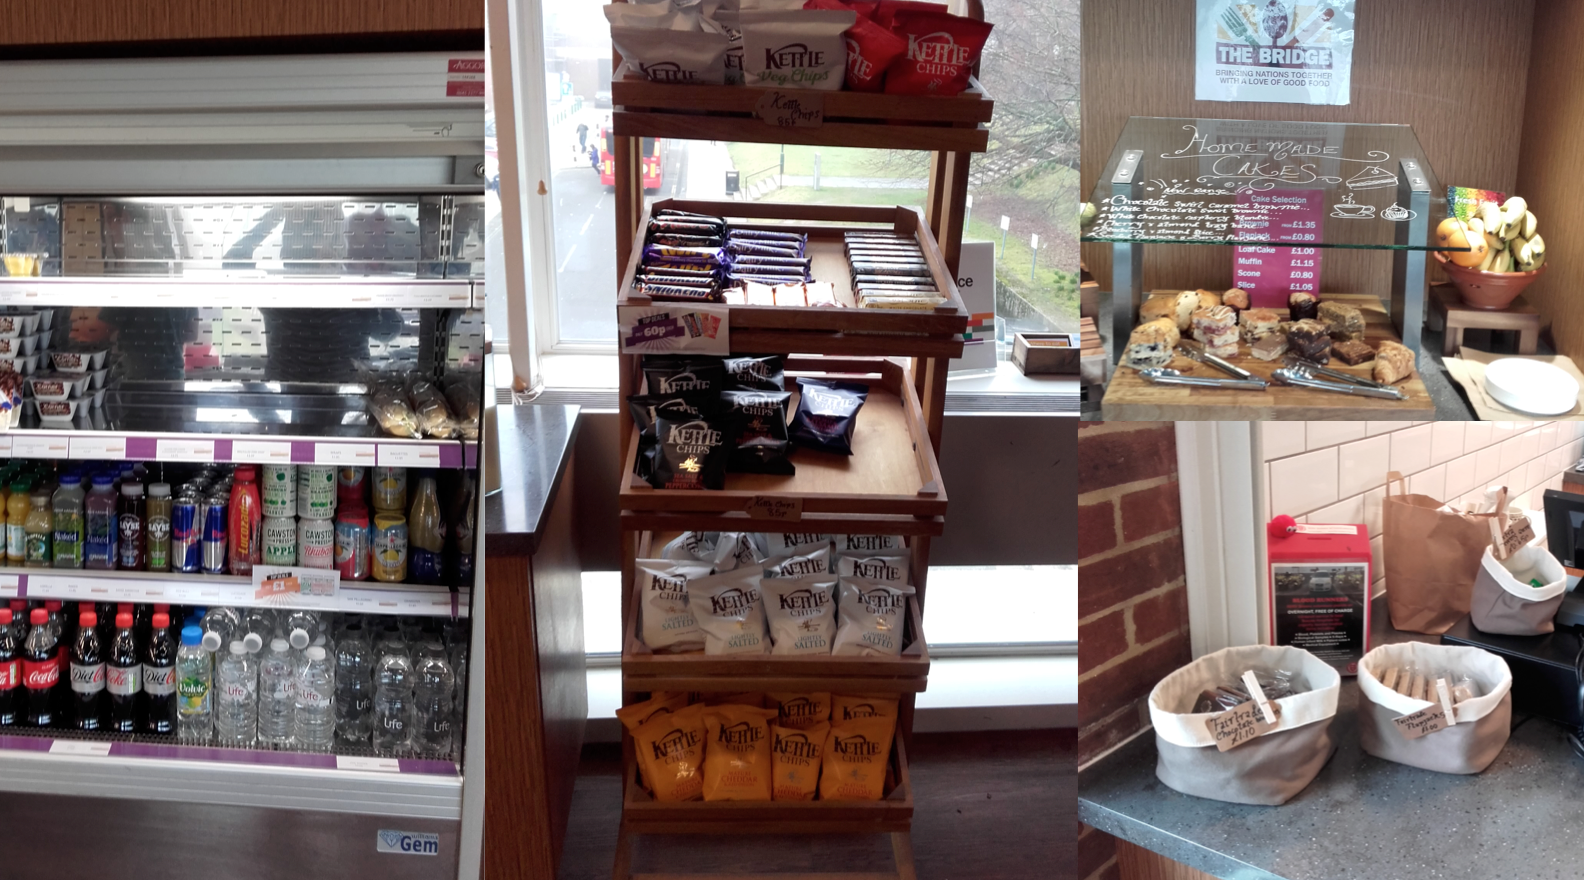
\includegraphics[width=14cm]{Figures/bridgePython.png}
% 	\caption{The various ``modules'' in the Bridge Cafe}
% \label{fig:be3}
% \end{figure}

\noindent A quick overview of modules: 
\begin{itemize}
\item Standard Python contains many built in functions, but does not contain everything you will need in your coding future.
\item Modules can be added to Python and contain dozens of functions.
\item Occasionally (but rarely, this is mostly avoided) function names are duplicated in different modules or between standard Python and a module. Even though they share a name the operation of these functions could be very different. Therefore, you have to be careful to use the correct version (by specifying the module name explicitly in the function call).
\item You should only import the modules that you need, and only import them once (loading modules multiple times and/or loading modules you don't need leads to wasted RAM).
\end{itemize}

\begin{tcolorbox}[colback=red!5!white,colframe=red!75!black]
Terminology gets a bit muddy from here on out... strictly a function is a self defined chunk of reusable code, as you have seen in the previous chapter. These modules in fact contain "methods", a term which will make far more sense if you progress to object-orientated \texttt{Python}. For simplicity we will use the two interchangeably, mostly focusing on mis-using "function" but don't be confused if you come across "method" in the future or online.
\end{tcolorbox}

\section{Common Python modules}

Modules we will cover in this course\footnote{We are using ``course'' rather than ``sub-module'' to avoid confusion with the topic of this lab session.} include: 
\begin{itemize}
\item {\tt matplotlib}: graphics tools to create and display plots. In Physics and Astrophysics it is frequently used to make plots for publications.
\item {\tt numpy}: data structures and mathematical resources not included in basic Python, for example cosine, exponentials etc. Some basics of {\tt numpy} will be discussed in this section but chapter \ref{chap:numpy} will provide a more comprehensive overview. 
\item  {\tt scipy}: scientific resources such as those needed in mathematical physics, e.g. bessel, gamma, beta functions, signal processing, integration, differential equation solving and statistics... (you will use {\tt scipy} a {\bf lot} in Scientific Computing in Y2).
\item  {\tt random} (Section~\ref{randommodule}): used to generate pseudo-random numbers within the Python environment. The module is very useful for generating random numbers quickly in a range of circumstances.
\item  {\tt pandas} (see Chapter~\ref{Chapter6}): allows you to work with data in something analogous to spreadsheets.
\item  {\tt os}: allows you to interface Python with Unix, for example if you want to load up certain types of file into your Python code.
\end{itemize}

%\item{\tt math} (Section~\ref{mathmodule}) does much the same as {\tt numpy} (and hence to the maths functions inside {\tt pylab}) so you probably won't need it. But occasionally {\tt numpy} will not have (or seem not to have) what you need, see example 3 in Section~\ref{INeedMaths}.
\newpage
\noindent Here are some additional modules that you may come across, especially if you are working on the optional challenges or an independent project. Although it is absolutely fine to use these, or other, non-standard modules in your optional work, please do not use them in the assessments.
%ADD MORE
\begin{itemize}
\item {\tt TkInter}: a way to use GUIs with Python.
\item {\tt PyGame}: if you are writing games.
\item {\tt SQLAlchemy}: if you want to set up a database.
\item {\tt SymPy}: Symbolic equation solving in python, this is essentially free Maple.
\item {\tt time}: amongst other things, this contains a useful function to check how long your code is taking to run.
\item  {\tt html}: write webpages in python.
\item {\tt astropy}: if you are lucky enough to do any astronomy research, then you'll definitely be using this one. It also contains an invaluable sub-module for working with and converting units, as well as another sub-module containing all the useful constants your heart could possibly desire.
\item \texttt{scikit learn}: a suite of simple machine learning algorithms.
\item \texttt{tensorflow}: a more in depth module filled with machine learning "machienery", including lots of GPU optimisation.
\end{itemize}

\noindent You can find many more modules described online, e.g. check out \\ {\tt https://wiki.python.org/moin/UsefulModules}

\section{Importing Modules}
\label{modload}
{\bf You should import all modules at the \underline{TOP} of your scripts: loading them anywhere else can quickly lead to confusion, i.e. DO NOT import modules in any other cell than the first in \texttt{jupyter}.}

There are several different ways of importing modules. The different methods have advantages and disadvantages based upon the task. Until you get more used to Python, you should keep checking with the ATs to make sure you are using the correct method. For now you'll be using one or more of the following methods in \texttt{jupyter}. When you become more proficient, you might well be driving python from the command line, or from inside a .py file, and you can load the modules in the same way for those.

\newpage

\subsection{Method One}
The simplest way to import a module is the following. This example shows how to import the \texttt{numpy}  module:
\begin{lstlisting}[style=PY]
import numpy
\end{lstlisting}
This method allows you to access all the functions in a module, without explicitly importing them into your code and using up your computer's RAM (Random Access Memory- the fast access memory used for running processes on your computer, not used to store data). To use a function from that module within the code, we need to tell python the function is associated with the module by joining the function to the module using a full stop, i.e. {\tt module.function}, e.g.:
\begin{lstlisting}[style=PY]
In[1]:  import numpy
        print(numpy.exp(1))
        print(numpy.pi)
\end{lstlisting}
\begin{lstlisting}[style=PY_out]
        2.718281828459045
        3.141592653589793
\end{lstlisting}

\subsection{Method Two}
This method imports the module with a custom name for use when calling upon functions, this saves time with modules with long names etc.
\begin{lstlisting}[style=PY]
In[2]:  import numpy as np
        print(np.exp(1))
        print(np.pi)
\end{lstlisting}
 Note that you are not obliged to use {\it np} as the short version for the {\tt numpy} module. You could use {\it daffodil} if you wanted, but of course you'd not save any time that way! Also note that you can still use the full name of the module, in addition to the short hand. You will find that there are accepted names for a huge number of commonly used modules such as np:numpy, plt:matplotlib, tf: tensorflow etc.

\subsection{Method Three}
The third method imports all the functions from a module into Python for use.
\begin{lstlisting}[style=PY]
In[3]:   from numpy import *
\end{lstlisting}
This simply tells Python, to import all functions from numpy. To then call upon the function just type the function name:
\begin{lstlisting}[style=PY]
In[4]:  print(exp(1))
        print(pi)
\end{lstlisting}
\begin{lstlisting}[style=PY_out]
        2.718281828459045
        3.141592653589793
\end{lstlisting}
The main disadvantages of this method are that you will waste memory (RAM) and, when importing multiple modules, you might be importing similar functions with the same names. You then have to take extra care to make sure you are using the function you intended.
\vspace{0.25cm}
\begin{tcolorbox}[colback=red!5!white,colframe=red!75!black]
\textbf{Do not use Method three}. It wastes memory, time, and can potentially cause massive conflicts with other modules, if you're importing more than one; it is bad Python practice. Using abrreviations, or more officially: ``namespaces'', like \texttt{np} makes the code easier to read, allows other developers to know where the function comes from, and most importantly only loads it into memory when the function is actually used.
\vspace{0.25cm}

Method three has been described here purely so that you are aware of its potential use, especially when looking online for help. 
\end{tcolorbox}

\subsection{Method Four}
The fourth method is similar to the third method, however this time you can specify which functions from a module you wish to use - this method is often the best method when you only want to use one or two functions from a library.

\noindent \textbf{Please restart your kernel now}.
\begin{lstlisting}[style=PY]
In[1]:  from numpy import exp,sin
\end{lstlisting}
You can import as many of the functions as you like from the module all separated by a comma. 
\begin{lstlisting}[style=PY]
In[2]:  print(exp(1))
        print(sin(3.14)) #note that Python defaults to radians
\end{lstlisting}
\begin{lstlisting}[style=PY_out]
        2.718281828459045
        0.0015926529164868282
\end{lstlisting}
\vspace*{1ex}
\noindent If you try to use a function you did not import a NameError will occur, e.g. try:
\begin{lstlisting}[style=PY]
In[3]:   print(pi)
\end{lstlisting}
\begin{lstlisting}[style=PY_out]
---------------------------------------------------------------------------
NameError                                 Traceback (most recent call last)
<ipython-input-15-9e2d2bd32686> in <module>
----> 1 print(pi)

NameError: name 'pi' is not defined
\end{lstlisting}

\newpage

\section{Accessing help with modules and functions}

\subsection{The {\tt dir} command}

To find what functions are within a module we can use the {\tt dir} function. For example, the following shows the contents of the {\tt random} module (note that only the last part of the {\tt dir(random)} response is shown):   
\begin{lstlisting}[style=PY]
In [4]: import random
        dir(random)
\end{lstlisting}
\begin{lstlisting}[style=PY_out]
Out[4]: .....
        'randint',
        'random',
        'randrange',
        'sample',
        'seed',
        'setstate',
        'shuffle',
        'triangular',
        'uniform',
        'vonmisesvariate',
        'weibullvariate']
\end{lstlisting}

\noindent So using the {\tt dir} command enables us to learn about a module. 

\subsection{The {\tt help} command}
In a Python command line, typing \texttt{help( )} with a function name in between the parentheses will display a help file about that function (if it exists). In the example below, we look for information on the range function (only the first part of the {\tt help(range)} response is shown):

\begin{lstlisting}[style=PY]
In [5]: help(range)
\end{lstlisting}

\begin{lstlisting}[style=PY_out]
Out[5]: Help on class range in module builtins:

        class range(object)
         |  range(stop) -> range object
         |  range(start, stop[, step]) -> range object
\end{lstlisting}

\noindent If you mistype a function name, you will get a {\tt NameError}. See what happens when you type {\tt help(renge)}.

\noindent The help command will tell you what inputs you have to give to the function, as well as any that are optional. If you see a function with parameters in square brackets, [], then these input are optional. Do not type the function out with the square brackets as you see in the help screen, you'll get a syntax error:

%\begin{verbatim}
\begin{lstlisting}[style=PY]
In [6]: range([1,]40[,2])
\end{lstlisting}
\begin{lstlisting}[style=PY_out]
Out[6]: File "<ipython-input-19-da85a1b3f88c>", line 1
        range([1,]40[,2])
              ^
        SyntaxError: invalid syntax
\end{lstlisting}

\subsubsection{When {\tt help()} is not actually helpful}

Python is free, and sometimes the help pages reflect this, i.e. they are not useful, especially for beginners. For example, try {\tt help(sin)} (you need to have loaded it from {\tt numpy} first). If you get stuck and {\tt help()} doesn't help, then don't despair! You can ask your AT, or Google, or StackOverflow, or a friend for help.

\noindent A quick sidenote, taking breaks definitely helps when you are coding. Sometimes, you need to go to sleep for the solution to a problem to show itself. Also, make sure you don't suffer alone, complain about your issues to your friends, sometimes talking about the problem can help the solution pop up. In fact, a very helpful process in coding called "rubber ducking" involves chatting rubbish to an inanimate object until the issue resolves itself in your head, feel free to substitute the inanimate object for a weary friend. Sometimes talking through the problem is all you need.

\subsection{Exercises}

\subsubsection{Exercises (with worked solutions)}
\label{INeedMaths}
\noindent These exercises require the {\tt numpy} module. Please try to figure out which functions to use and how to use them by yourself (make use of the numpy documentation and the \texttt{help} function) before checking the answers (section~\ref{workedanswersCh5}). Learning how to figure out how to do things in Python that you've not been explicitly taught is an essential skill.\\

Compute the following:
\begin{enumerate}
\item $\sin(\frac{\pi}{3})$
\item $\frac{\log(100)}{\log(10)}$
\item Convert 60 degrees to radians.
\item $\log_2(6)$
\item ln(5)
\item Check if $4\times\arctan(1)$ is equal to $\pi$ (print True or False)
\end{enumerate}


\subsubsection{Exercises (other)}
\begin{enumerate}
    \item W5Basic1 - Write a function that checks Euler's formula,
    \[
    e^{\pm i\theta}=\cos \theta \pm i \sin \theta,
    \]
    for any argument $\theta$.
    \begin{enumerate} 
        \item Check that the right hand side is equal to the left hand side.
        \item It must return True if the formula holds.
    \end{enumerate}

\item W5Basic2 - Evaluate $\log_6(2)$ (hint: use the logarithm base change rule).
\end{enumerate}

\section{The {\tt random} module}
\label{randommodule}

In Physics research and statistics, random numbers are used all the time for many purposes; from making random sub-samples of a large dataset to helping us sample highly complex mathematical functions. In this course we'll use randomly generated numbers from a uniform (all numbers in range equally possible) probability distribution and from a Normal (or Gaussian) probability distribution.

\subsection{Exercises}

\subsubsection{Exercises (with worked solutions)}
\label{W5EWWS2}
\noindent Now it's time for some self-driven learning, using the skills taught above: \texttt{dir}, \texttt{help} and indeed the internet which no programmer ever works without, try these exercises. (for answers see section~\ref{workedanswersCh5}).
\begin{enumerate}
\item Investigate the {\tt randint, randrange, random}, {\tt uniform} functions, and {\tt gauss}.
\item Generate a random number.
\item Generate a random number between 1 and 10.
\item Generate a random integer between 1 and 100.
\item Generate 100 random numbers from a normal distribution with $\mu=5$ and $\sigma=2$ and store them in a list.
\end{enumerate}

\subsubsection{Exercises (other)}

\begin{enumerate}
    \item W5Basic3 - Write a function that displays a random letter from an inputted name.
    \item W5Basic4 - Generate a random number between 1 and 100 that is divisible by 9. Hint: use {\tt random.randrange}.
\end{enumerate}

\begin{tcolorbox}[colback=red!5!white,colframe=red!75!black]
\subsection{Seeding}
Often when working with random numbers we may want random numbers but also repeatable results for debuggig/testing. Now... this seems a little paradoxical but it is a very real requirement which you will undoubtedly encounter at some point. To achieve this we can simply "seed" our random numbers. To do this with \texttt{random} we simply employ the seed function:

\begin{lstlisting}[style=PY]
In [7]: random.seed(1)
\end{lstlisting}

Now our random numbers will be the same sequence regardless of when we run it. The only requirement of seed is that the argument (1 here) is an integer, this integer can be any integer and defines the random sequence deterministically. If no seed is set the random numbers are simply seeded by the current system time in milliseconds (ticks) from 1970.
\end{tcolorbox}

\section{The {\tt arange} command}

The \texttt{arange} function is part of the {\tt numpy} module. You can think of it as an advanced version of the built in \texttt{range} function (refer back to section~\ref{sec:range}). Unlike the regular \texttt{range} function, the \texttt{arange} function allows floats, so you can have step sizes of 0.5 or 0.1, etc. The function doesn't return a vanilla Python list, but instead a numpy array (the difference is akin to that between a vector and a matrix, for more see Chapter \ref{chap:numpy}).
\begin{lstlisting}[style=PY]
In[8]:  from numpy import arange
        x = arange(1, 10.5, 0.5)
\end{lstlisting}

\noindent The above generates an array from 1 to 10 in intervals of 0.5. The command is very similar to \texttt{range} and the same argument layout can be inferred. Below are some of the outputs using the \texttt{arange} function. Try all of these in your Jupyter notebook.
\begin{lstlisting}[style=PY]
In [1]: arange(4.0)
\end{lstlisting}
\begin{lstlisting}[style=PY_out]
Out[1]: array([0., 1., 2., 3.])
\end{lstlisting}
\begin{lstlisting}[style=PY]
In [2]: arange(2, 5)
\end{lstlisting}
\begin{lstlisting}[style=PY_out]
Out[2]: array([2, 3, 4])
\end{lstlisting}
\begin{lstlisting}[style=PY]
In [3]: arange(1, 2, 0.25)
\end{lstlisting}
\begin{lstlisting}[style=PY_out]
Out[3]: array([1., 1.25, 1.5 , 1.75])
\end{lstlisting}

\noindent Table \ref{tab:arc} summarises the options available with the arange function.
\begin{table}
\begin{center}
\begin{tabular}{|l | p{7cm}|}
\hline
\texttt{arange(j)} & Creates an array starting at 0 and ending at \texttt{j-1} with increments of 1\\\hline
\texttt{arange(i, j)} & Creates an array starting at \texttt{i} and ending at \texttt{j-1} with increments of 1\\\hline
\texttt{arange(i, j, k)} & Creates an array starting at \texttt{i} and ending at the nearest number to \texttt{j} based on the increments of \texttt{k}\\\hline
\end{tabular}
\end{center}
\caption {How to use the {\tt arange} command}
\label{tab:arc}
\end{table}\\

\newpage
\section{The \texttt{matplotlib.pyplot.plot} function}

The {\tt matplotlib} module is commonly used to make graphs and figures in Python, it is very easy to use and with some practise can make publication quality plots. Below is an example of how to plot the simplest mathematical equation, $y=x$.
\begin{lstlisting}[style=PY]
In[8]:  import matplotlib.pyplot as plt

        # Set up variables for plotting
        x = np.arange(1, 5.5, 0.5)
        y = x
        
        # Plot the variables
        plt.plot(x, y)
        plt.show()
\end{lstlisting}
The initial line of the code imports the {\tt pyplot} package from matplotlib. Then the \texttt{arange} command creates a range of $x$ values from 1 to 5 in increments of 0.5. The \texttt{y=x} line just links the variable name $y$ to the $x$ variable. The \texttt{plot} command then generates a line plot. However, this just generates the line on internal matplotlib "figure", to see it we need to \texttt{show()} it. This is done with the \texttt{show()} command which displays the plot on screen. The output can be seen in figure \ref{fig:pyx}.

\begin{figure}[H]
	\centering
	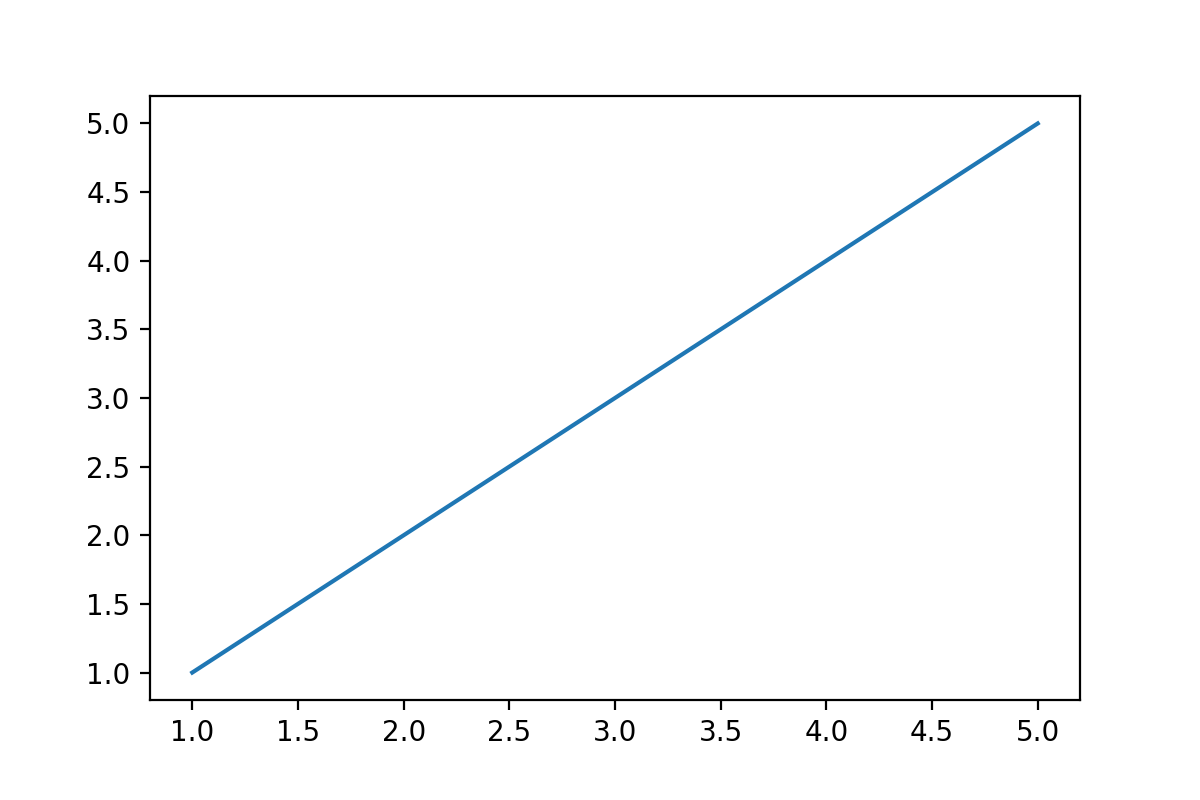
\includegraphics[height=10cm]{Figures/plotyx.png}
\caption{Plot of $y=x$.}
\label{fig:pyx}
\end{figure}

You may have noticed a little fib here... in \texttt{jupyter} the plot is shown regardless of whether {\tt plt.show()} is called. This is for the same reason that the print function isn't required to print variables, thus it isn't true when not using \texttt{jupyter}, you should therefore get in the habit of using {\tt plt.show()}... it is more correct after all.

You can also change the limits of the graph. Below is an example of $y=x^{2}$, with set limits. The output is shown in Figure \ref{fig:pyx2}.
\begin{lstlisting}[style=PY]
In[9]:  # Set up a range of x values
        x = np.arange(-5, 5, 0.01)
        
        # Compute the square of the x values
        y = x**2
        
        # Plot the result
        plt.plot(x, y)

        # Set axis limits
        plt.xlim(-1, 2)
        plt.ylim(-1, 5)

        plt.show()
\end{lstlisting}

\texttt{xlim} and \texttt{ylim} set the limits, and they need to come after the \texttt{plot} command, but before the \texttt{show} command, as \texttt{plot} draws the plot, then the limits are added before the graph is shown on screen.

\begin{figure}[H]
	\centering
	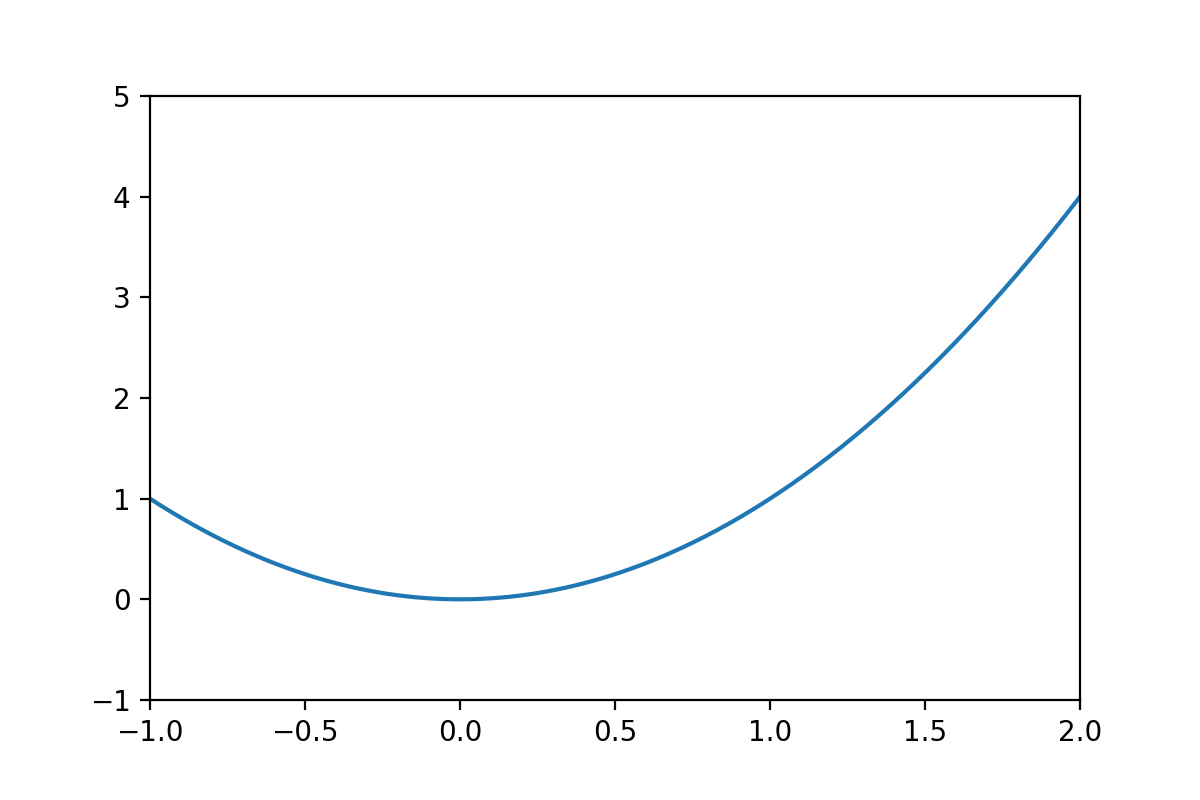
\includegraphics[height=10cm]{Figures/plotyx2.png}
\caption{Plot of $y=x^{2}$.}
\label{fig:pyx2}
\end{figure}

Additionally you can add labels to your axis and a title to your graph. Below is an example of $y=\sin(x)$.
\begin{lstlisting}[style=PY]
In[10]: # Set up a range of x values
        x = np.arange(-20, 20, 0.001)
        
        # Compute the sin of these values
        y = np.sin(x)
        
        # Plot the result
        plt.plot(x, y)

        # Set a title and label the axes
        plt.title('Graph of y = sin(x)')
        plt.xlabel('This is the x axis')
        plt.ylabel('This is the y axis')

        # Draw lines to mark 0 on the x and y axes
        plt.axhline(0, color='black', linestyle='--')
        plt.axvline(0, color='black', linestyle='--')

        # Set the y-axis limits
        plt.ylim(-1.2, 1.2)

        plt.show()
\end{lstlisting}

\noindent Just as when adding limits to the plot, any commands to set titles or labels have to come after the initial \texttt{plot}. \texttt{title}, \texttt{xlabel}, and \texttt{ylabel} are pretty self explanatory; you have to pass your chosen title/label as a string, which is then added to the plot (these can include \LaTeX formatting, i.e. {\tt $y=\sin(x)$}). The \texttt{axhline} (for horizontal lines) and \texttt{axvline} (for vertical lines) add \texttt{y=0} and \texttt{x=0} axis to your graph. Here we have added a dashed line by setting the \texttt{linestyle} argument. The plot produced by this code can be seen in Figure \ref{fig:pysinx}.

\begin{figure}[H]
	\centering
	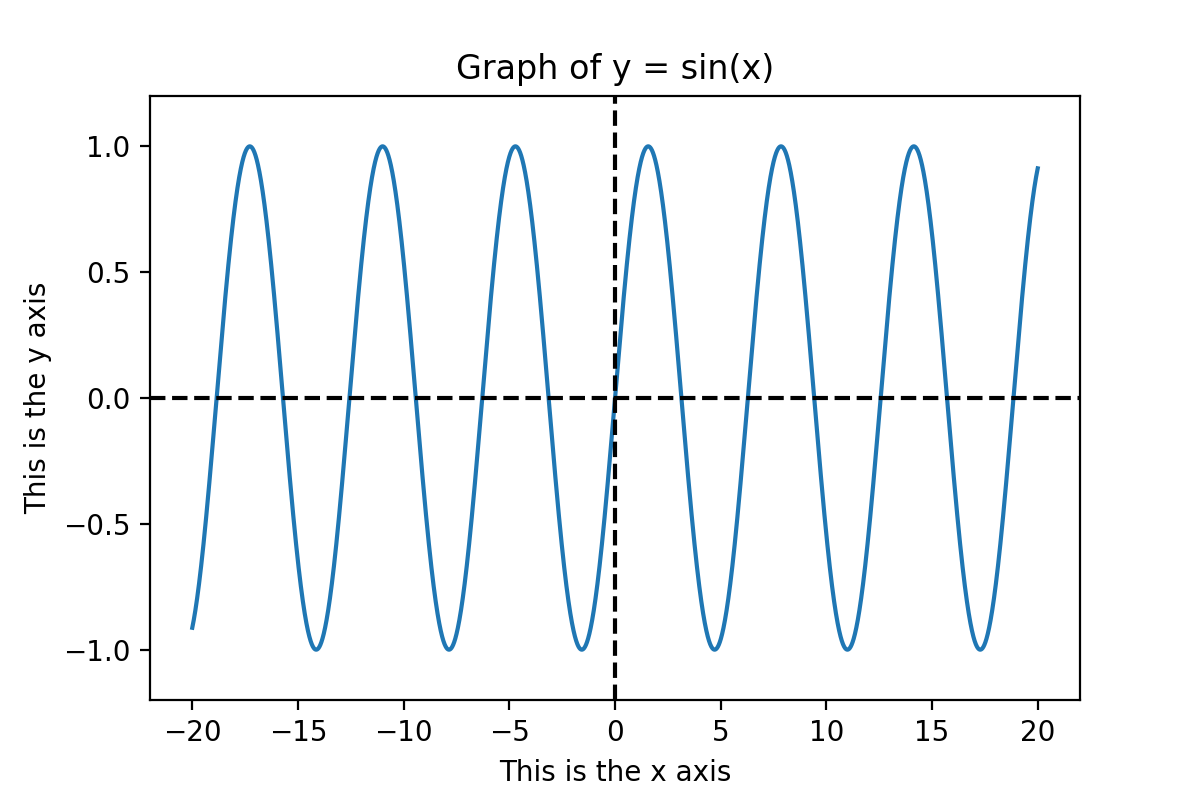
\includegraphics[height=10cm]{Figures/plotysinx.png}
\caption{Plot of $y=\sin(x)$.}
\label{fig:pysinx}
\end{figure}

\subsection{Exercises}
\begin{enumerate}
    \item W5Basic5 - Plot a graph of $\cos(x)$
    \item W5Basic6 - Plot a graph of $\cosh(x-20)$
    \begin{enumerate}
        \item Limit the x-axis to between $-20$ to $5$.
        \item Add an appropriate title, set the fontsize to 14.
    \end{enumerate}
    \item W5Basic7 - Plot a Gaussian distribution with mean of 0 and a variance of 1.
    \begin{enumerate}
        \item Look up the equation for the Gaussian probability density function.
        \item Generate some x values between -3.2 and 3.2, then use the equation to calculate the equivalent y-values.
        \item Plot the Gaussian, and add an appropriate title.
    \end{enumerate}
\end{enumerate}

\section{Plotting in multiple figures}
When you have more than one graph to display, you have to use the \texttt{figure} function. This allows you to separate what you're plotting, otherwise everything will end up on the same set of axes. In the example below we generate two plots and display both below one \texttt{jupyter} cell, give it a try.
\begin{lstlisting}[style=PY]
In[11]: # Generate a range of x values, with a small step size
        x = np.arange(-20, 20, 0.001)  
        
        # Create figure with id 1
        plt.figure(1)
        
        # Calculate the sin of all the x values
        y_sin = np.sin(x)
        
        # Plot the result in figure 1
        plt.plot(x, y_sin)
        
        # Add a title to figure 1
        plt.title('Graph of y = sin(x)')
        
        # Set the y limit for figure 1
        plt.ylim(-1.2, 1.2)
        
        # Create figure with id 2
        plt.figure(2)
        
        # Compute the cosine of the x values
        y_cos = np.cos(x)
        
        # Plot the result in figure 2
        plt.plot(x, y_cos)
        
        # Add a title to figure 2
        plt.title('Graph of y = cos(x)')
        
        # Set the y limits of figure 2
        plt.ylim(-1.2, 1.2)
        
        plt.show()
\end{lstlisting}

\noindent Once you've plotted something, you're also able to close it; this can be particularly useful if you're creating a very large set of plots, as they can start to slow down your computer. To close every open plot, you can use \texttt{plt.close("all")}, or if you only wanted to close the first plot from the above example, we could run \texttt{plt.close(1)}.

% \begin{figure}
% 	\centering
% 	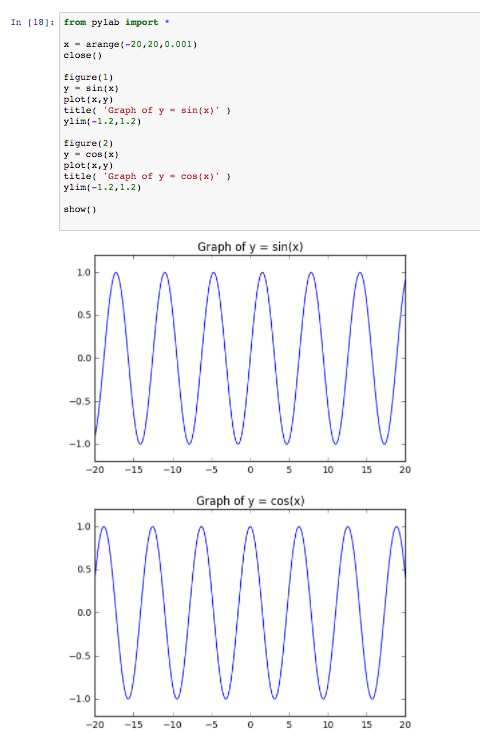
\includegraphics[width=10cm]{Figures/SinCosPlot.png}
% \caption{Plot of $y=\sin(x)$ in one window and $y=\cos(x)$ in the other.}
% \label{fig:sinxcosx}
% \end{figure}

\section{Plotting a Scatter with \texttt{plt.scatter}}

Often you will have data that doesn't lend itself to plotting with a nice line. Instead you'll need to plot a scatter of points and maybe plot a theory as a line overlaid over the top. Lets use some of what we learnt with the random module to create a nice messy scatter plot. This can be achieved using {\tt plt.scatter}.

\begin{lstlisting}[style=PY]
In[12]: # Initialise lists to store x and y values
        x = []
        y = []
        
        # Loop getting 500 random numbers between 1 and 10
        for i in range(500):
            x.append(random.uniform(1, 10))
        
        # Loop again but this time use a while loop (theres no difference)
        i = 0
        while i < 500:
            y.append(random.uniform(1, 10))
            i += 1
        
        # Plot the resulting scatter
        plt.scatter(x, y, marker='+')
        
        # Add a title
        plt.title('My Mess')
        
        # Label the axes with latex
        plt.xlabel('$x$')
        plt.ylabel('$y$')
        
        # Add a grid
        plt.grid(True)
        
        plt.show()
\end{lstlisting}

Here we have simply extracted 500 random numbers from a uniform distribution and plotted them with "+"s. This marker argument can be a number of things, for a full list look online or in Tab. \ref{tab:plte}, some examples include {\tt '.', ',', 'o'} and {\tt '+'} used here. By default it uses circles (\texttt{'o'}). We have also employed the use of \LaTeX\ math mode in the labels and drawn a grid on the background, this can make plots easier to read and is often recommended. The output is shown in Figure \ref{fig:mess}.

\begin{figure}[H]
	\centering
	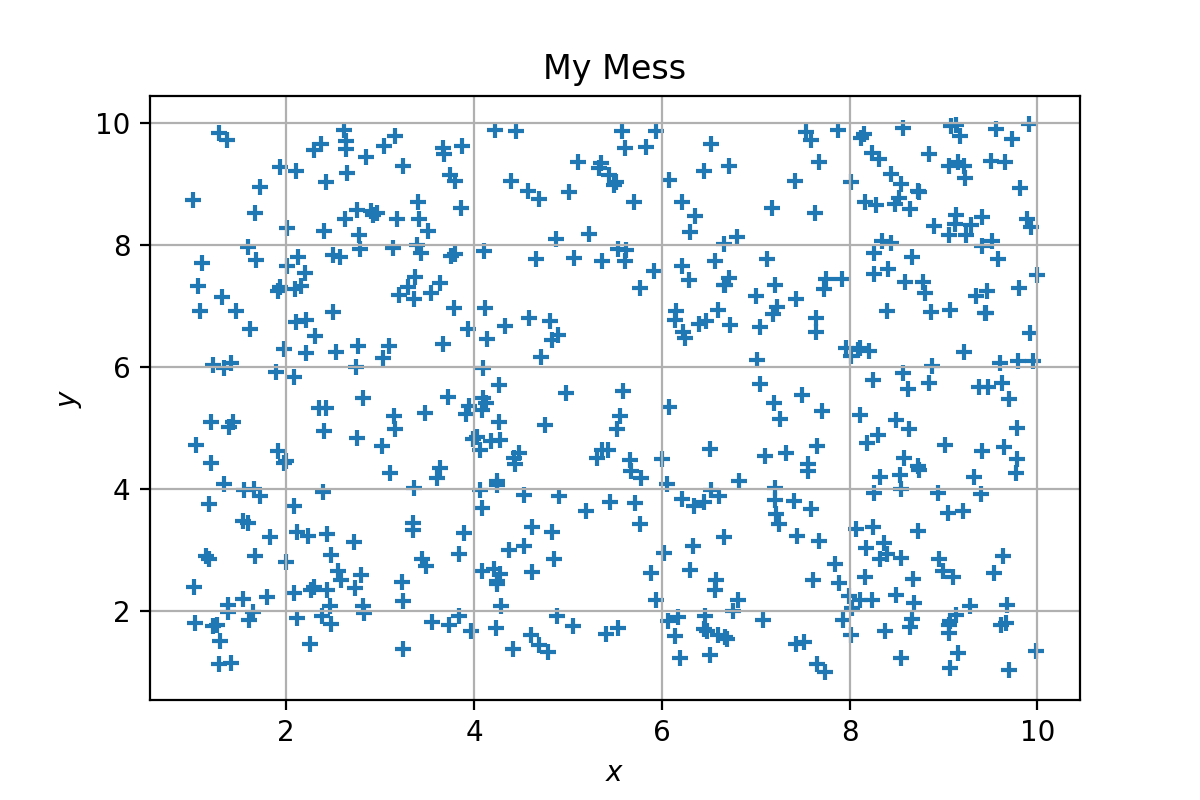
\includegraphics[width=\linewidth]{Figures/plotmess.png}
\caption{An example scatter plot.}
\label{fig:mess}
\end{figure}

\subsection{Exercises}

\begin{enumerate}
    \item W5Basic8 - Write a code that makes two figures
    \begin{enumerate}
        \item Limit both figures to $-5$ to $5$ on the x-axis, and $-1.2$ to $1.2$ on the y-axis.
        \item Plot $\sin(2x+1)$ on the first figure.
        \item Plot $\cos(2x+1)$ on the second figure.
        \item Make sure to give both plots appropriate titles, x-axis labels, and y-axis labels.
    \end{enumerate}
\end{enumerate}

\section{Signpost}

You should have got to at least this point by the end of Session 5. By now you have the tools to complete parts a) to c)  of the second assessment. If you have time at the end of Session 5 we suggest you work through the advances exercises.

\section{Advanced Exercises}
\label{ExAdw5}

\begin{enumerate}
\item Use the random module to create a coin flip simulator. Flip the coin 100 times and print out how many times it landed on heads, and how many times on tails (think about what the results should be before you run it).
\item Plot $\sin(x)$ and $\cos(x)$ on the same graph, with limits $-10$ to $10$ on the x-axis.
\item Plot $\sin^{2}(x)-\cos(x)$ with limits $1$ to $5$ on the x-axis and $0.9$ to $1.3$ on the y-axis. Change the line colour to yellow and line width to 5 (use \texttt{help} and/or the matplotlib documentation).
\item Imagine you have some scattered data with a linear relation. Write your own function that naively computes the values \texttt{m} and \texttt{c} from $y=mx+c$ for a 1 dimensional linear line of best fit.
\item Use the gauss function from the random module to generate 1000 numbers from a Gaussian distribution with a mean of zero and a variance of one, then plot the data as a histogram with one hundred bins. Hint: Use the pyplot.hist command instead of pyplot.plot.
\end{enumerate}


\section{Worked Examples}
\label{workedanswersCh5}

\noindent These are the solutions for section \ref{INeedMaths}:
\begin{lstlisting}[style=PY]
In[1]:  # Question 1
        print(np.sin(np.pi/3))
\end{lstlisting}
\begin{lstlisting}[style=PY_out]
Out[1]: 0.8660...
\end{lstlisting}

\begin{lstlisting}[style=PY]
In[2]:  # Question 2
        print(np.log(100)/np.log(10))
\end{lstlisting}
\begin{lstlisting}[style=PY_out]
Out[2]: 2.0
\end{lstlisting}

\begin{lstlisting}[style=PY]
In[3]:  # Question 3
        print(np.radians(60))
\end{lstlisting}
\begin{lstlisting}[style=PY_out]
Out[3]: 1.047... 
\end{lstlisting}

\begin{lstlisting}[style=PY]
In[4]:  # Question 4
        print(np.log2(6))
\end{lstlisting}
\begin{lstlisting}[style=PY_out]
Out[4]: 2.584...
\end{lstlisting}

\newpage
\begin{lstlisting}[style=PY]
In[5]:  # Question 5
        print(np.log(5))
\end{lstlisting}
\begin{lstlisting}[style=PY_out]
Out[5]: 1.609... 
\end{lstlisting}

\begin{lstlisting}[style=PY]
In[6]:  # Question 6
        print(4*np.arctan(1)==np.pi)
\end{lstlisting}
\begin{lstlisting}[style=PY_out]
Out[6]: True
\end{lstlisting}

\noindent These are the solutions for section \ref{W5EWWS2}:
\begin{lstlisting}[style=PY]
In[1]:  # Question 2
        import random
        print(random.random())
\end{lstlisting}

\begin{lstlisting}[style=PY]
In[2]:  # Question 3
        print(random.uniform(1.0,10.0))
\end{lstlisting}

\begin{lstlisting}[style=PY]
In[3]:  # Question 4
        print(random.randint(1,100))
\end{lstlisting}

\begin{lstlisting}[style=PY]
In[4]:  # Question 5
        lst = []
        for ind in range(100):
            lst.append(random.gauss(5,2))
\end{lstlisting}

